\documentclass[journal]{IEEEtran}

\usepackage{amsmath,amssymb,amsfonts}
\usepackage{graphicx}
\ifCLASSOPTIONcompsoc
\usepackage[caption=false,font=normalsize,labelfont=sf,textfont=sf]{subfig}
\else
\usepackage[caption=false,font=footnotesize]{subfig}
\fi
\usepackage{booktabs}
\usepackage{multirow}
\usepackage{siunitx}
\usepackage{tabularx}
\usepackage{url}
\usepackage{algorithm}
\usepackage{algpseudocode}
\usepackage{balance}
\usepackage[section]{placeins}

\graphicspath{{../figures/}{figures/}{figs/}}

% =========================
% Fill-in macros
% =========================
\newcommand{\NumBands}{16}
\newcommand{\TileSize}{16}
\newcommand{\NumTrain}{24}
\newcommand{\NumVal}{8}
\newcommand{\PatchH}{128}
\newcommand{\PatchW}{128}
\newcommand{\NumSeeds}{3}

\newcommand{\PSNROSP}{34.463}
\newcommand{\SAMOSP}{7.460}
\newcommand{\SSIMOSP}{0.8861}

\newcommand{\PSNRExact}{34.756}
\newcommand{\SAMExact}{7.060}
\newcommand{\SSIMExact}{0.8992}

\newcommand{\PSNRLearn}{38.142}
\newcommand{\SAMLearn}{5.019}
\newcommand{\SSIMLearn}{0.9413}

\newcommand{\DeltaExactPSNR}{+0.293}
\newcommand{\DeltaExactSAM}{-0.400}
\newcommand{\DeltaLearnPSNR}{+3.679}
\newcommand{\DeltaLearnSAM}{-2.441}

\newcommand{\TimeOSP}{TBD}
\newcommand{\TimeExact}{TBD}
\newcommand{\TimeLearn}{TBD}

\title{A Fair and Interpretable Comparison of Fixed OSP, Discrete Exact OSP Selection, and OSP-Seeded Learnable MSFA for Snapshot Multispectral Demosaicking}

\author{
\centering
\begin{minipage}[t]{0.40\textwidth}
  \centering
  \IEEEauthorblockN{Dhruva V}\\
  \IEEEauthorblockA{Indian Institute of Information Technology Vadodara\\
  202351032@iiitvadodara.ac.in}
\end{minipage}
\hspace{0.06\textwidth}
\begin{minipage}[t]{0.40\textwidth}
  \centering
  \IEEEauthorblockN{Ayush Singh}\\
  \IEEEauthorblockA{Indian Institute of Information Technology Vadodara\\
  202351017@iiitvadodara.ac.in}
\end{minipage}
\thanks{This manuscript is an extended pre-submission draft prepared in IEEE journal style.}
}

\begin{document}
\maketitle

\begin{abstract}
Snapshot multispectral imaging offers compact acquisition hardware but introduces a challenging inverse problem due to sparse band-wise sampling. The sensing pattern, implemented as a multispectral filter array, strongly affects reconstruction quality and stability. Prior comparisons between fixed and learnable pattern design are frequently confounded by inconsistent data splits, unequal training schedules, or changing reconstruction backbones. This work presents a unified and controlled benchmark that compares three sensing branches under matched conditions: fixed optimal sphere packing (OSP), discrete Exact OSP selector, and OSP-seeded learnable MSFA. The fixed branch follows deterministic OSP generation with explicit tie-handling rules to preserve reproducibility. The Exact branch optimizes a discrete candidate distribution over valid OSP-derived tiles and then commits to a hard selected tile for refinement. The learnable branch initializes from OSP structure and optimizes soft sensing masks with a regularized objective that balances reconstruction quality, spatial-spectral dispersion, and interpretability. All branches share identical train and validation partitions, the same UNet demosaicking model, and aligned optimization protocols. The resulting analysis shows a clear progression in reconstruction quality from fixed OSP to Exact OSP to OSP-seeded learnable sensing while preserving transparent pattern semantics. The proposed pipeline provides a reproducible bridge between deterministic sensing design and adaptive data-driven optimization.
\end{abstract}

\begin{IEEEkeywords}
Multispectral imaging, demosaicking, snapshot sensing, filter array design, interpretable learning.
\end{IEEEkeywords}

\section{Introduction}
Multispectral imaging is useful in applications such as inspection, remote sensing, biomedical analysis, and material recognition because it records wavelength-dependent information that is not available in standard RGB imagery \cite{ghamisi2017,lu2014,wang2021}. Snapshot camera designs make such acquisition more compact by placing spectrally selective filters directly on the sensor in a fixed mosaic arrangement \cite{bayer1976,miao2006,geelen2014}. The practical advantage is hardware simplicity and single-shot capture, but the computational cost is that a dense spectral cube must be reconstructed from sparse band-wise samples.

In snapshot multispectral imaging, sensing and reconstruction should be analyzed together. Prior studies on MSFA design and demosaicking show that sampling layout influences reconstruction difficulty, while reconstruction quality also depends on the model used to invert the mosaic measurements \cite{hirakawa2008,jia2016,cheng2021,wu2021}. Therefore, improvements reported in demosaicking are most informative when the sensing strategy and reconstruction setting are discussed jointly.

Classical multispectral filter array design methods are deterministic and physically interpretable. They provide reproducible layouts and often rely on geometric criteria, including spatial-spectral dispersion objectives \cite{hirakawa2008,jia2016}. By contrast, data-driven sensing methods optimize the acquisition pattern jointly with reconstruction and can improve task performance, although the resulting masks can be harder to interpret when constraints are weak \cite{rueda2015,correa2015,arguello2014,mejia2018}.

A major practical issue is fairness of comparison. When architecture, warm-start availability, data protocol, or optimization budget vary at the same time, it becomes difficult to attribute performance changes specifically to sensing flexibility.

This paper addresses that gap through a strictly controlled comparison protocol among three branches:
\begin{enumerate}
\item Fixed OSP baseline with deterministic generation and deterministic tie handling.
\item Exact OSP selector over a valid discrete candidate bank derived from OSP construction.
\item OSP-seeded learnable MSFA with regularized soft-to-hard optimization.
\end{enumerate}

The core principle is simple: hold data, backbone, and training discipline constant, and vary only sensing design flexibility. This produces a cleaner interpretation of where performance gains come from.

Beyond protocol fairness, the methodological novelty is a unified sensing-design framework that spans deterministic, discrete-trainable, and continuous-trainable regimes under one constrained optimization view. In this framing, fixed OSP is a singleton feasible set, Exact OSP is a simplex-relaxed discrete search with deterministic hard commit, and the learnable branch is a prior-constrained differentiable sensing model with interpretable regularization.

\textbf{Main contributions are as follows.}
\begin{enumerate}
\item A reproducible fixed OSP baseline with deterministic tie-break semantics.
\item A deeper Exact OSP selector with complexity-aware discrete search, convergence diagnostics, and deterministic hard-commit semantics that remain interpretable.
\item A formal prior-constrained differentiable sensing framework for OSP-seeded learnable MSFA, combining interpretable priors with controlled adaptation.
\item A fair benchmark protocol with shared train and validation splits, shared U-Net backbone \cite{ronneberger2015}, matched schedules, and consistent metrics.
\item An ablation protocol and sensitivity analysis over key controls ($\lambda_{\mathrm{sp}}$, $\lambda_{\mathrm{ent}}$, $\alpha$, and $\tau$) to separate contribution of each design component.
\item A contextual discussion against external method families with clear protocol-mismatch caveats.
\end{enumerate}

\section{Related Work}
Research on multispectral demosaicking has progressed along two closely linked dimensions: sensing-pattern design and reconstruction modeling \cite{miao2006,hirakawa2008,cheng2021}. The first determines how spectral information is sampled at acquisition time, while the second determines how missing bands are inferred from sparse measurements. Although these dimensions are often studied separately, practical performance depends on their interaction.

\subsection{Snapshot Multispectral Sensing and MSFA Design}
Snapshot multispectral cameras typically use a multispectral filter array (MSFA) that tiles band-pass filters across the sensor plane. Compared with scanning systems, this design is compact and fast, but each pixel measures only one spectral band, leading to severe under-sampling. Classical and practical MSFA designs include binary-tree layouts, sensor-integrated mosaics, and reconstruction-aware variants \cite{miao2006,geelen2014,tsagkatakis2019}.

Distance-based design principles are natural for improving sampling diversity in a joint spatial-spectral space. Sphere-packing theory and lattice geometry provide a strong foundation for such formulations \cite{kepler2010,hales2005,hales2017,conway2013}. These methods are deterministic, interpretable, and reproducible, which is attractive for hardware-oriented benchmarking.

\subsection{Classical Demosaicking for Multispectral Data}
Before deep learning, multispectral demosaicking commonly relied on interpolation and channel-correlation modeling, including weighted bilinear interpolation, scattered-data interpolation, and iterative spectral-difference strategies \cite{brauers2006,amidror2002,mizutani2014}. These methods primarily exploit spatial smoothness within each band and correlation across nearby wavelengths \cite{brauers2006,mizutani2014}.

Frequency-domain CFA/MSFA analyses also showed that sensing-pattern design and reconstruction behavior are coupled \cite{hirakawa2008,jia2016}. This coupling motivates joint treatment of sensing and reconstruction when comparing methods.

\subsection{Deep Multispectral Demosaicking with Fixed Patterns}
Deep reconstruction methods improved quality under fixed sensing patterns by introducing stronger nonlinear priors and multiscale feature extraction \cite{cheng2021,wu2021}. These gains, however, do not by themselves isolate sensing-design quality, because decoder strength can partly mask acquisition weaknesses.

\subsection{Learnable Sensing and Joint Sensor-Decoder Optimization}
A major trend is joint optimization of coding and reconstruction in compressive and multispectral imaging pipelines \cite{rueda2015,correa2015,arguello2014,mejia2018}. Because the acquisition operator is adapted to the data distribution and decoder, such methods can outperform fixed sensing designs. The tradeoff is that unconstrained adaptation can reduce interpretability and deployment transparency if regularization and reporting discipline are weak.

\subsection{Structured and Hybrid Approaches}
Structured pattern optimization remains important in practice. Blue-noise-based coding and constrained coded-aperture design are representative examples in which additional structure is imposed to improve sampling behavior \cite{correa2016,lau2000,rodriguez2008}. These studies support the broader principle used here: preserve interpretable structure while allowing controlled adaptation.

\subsection{Evaluation Practice and Reproducibility Gaps}
Fair comparison becomes difficult when data splits, optimization budgets, and reported metrics are not aligned across methods. Public datasets and reproducible training procedures are therefore important ingredients for controlled evaluation \cite{yasuma2010,kingma2014}. Our framework is designed to reduce those confounders by enforcing shared protocol conditions across all sensing branches.

\section{Problem Formulation}

\subsection{Snapshot Multispectral Sensing Model}
Let $\mathbf{X}\in[0,1]^{K\times H\times W}$ denote a ground-truth multispectral cube with $K$ spectral bands, spatial height $H$, and width $W$. In snapshot sensing, only one spectral channel is measured per pixel according to an MSFA pattern.

Define a periodic tile of size $P\times P$ and corresponding one-hot masks
\begin{equation}
\mathbf{M}_k \in \{0,1\}^{H\times W},\quad k=1,\dots,K,
\end{equation}
with per-pixel one-hot constraint
\begin{equation}
\sum_{k=1}^{K}\mathbf{M}_k(i,j)=1,\quad \forall(i,j).
\end{equation}
The mosaicked measurement is
\begin{equation}
\mathbf{Y}=\sum_{k=1}^{K}\mathbf{M}_k\odot \mathbf{X}_k + \mathbf{N},
\label{eq:forward}
\end{equation}
where $\odot$ is elementwise multiplication and $\mathbf{N}$ is optional sensor noise.

\subsection{Reconstruction Objective}
A demosaicking network $\mathcal{R}_{\theta}$ maps the single-channel mosaic to a full spectral estimate:
\begin{equation}
\hat{\mathbf{X}}=\mathcal{R}_{\theta}(\mathbf{Y}).
\end{equation}
Given dataset $\mathcal{D}=\{\mathbf{X}^{(n)}\}_{n=1}^{N}$, the base reconstruction risk is
\begin{equation}
\mathcal{L}_{\mathrm{rec}}(\theta,\phi)=
\mathbb{E}_{\mathbf{X}\sim\mathcal{D}}
\left[
\ell\big(\mathcal{R}_{\theta}(\mathcal{S}_{\phi}(\mathbf{X})),\mathbf{X}\big)
\right],
\end{equation}
where $\mathcal{S}_{\phi}$ is the sensing operator induced by MSFA parameter $\phi$.

In this work, $\ell(\cdot)$ combines pixel, spectral-angle, and gradient consistency terms:
\begin{align}
\ell
=\;&
\lambda_{1}\mathcal{L}_{1}
+\lambda_{\mathrm{sam}}\mathcal{L}_{\mathrm{sam}}
+\lambda_{\mathrm{grad}}\mathcal{L}_{\mathrm{grad}}
+\lambda_{\mathrm{spec}}\mathcal{L}_{\mathrm{spec}}.
\label{eq:base_loss}
\end{align}

\subsection{Constrained Joint Optimization View}
All branches can be written as:
\begin{equation}
(\phi^{\star},\theta^{\star})=
\arg\min_{\phi\in\Phi,\theta}
\mathcal{L}_{\mathrm{rec}}(\theta,\phi)+\Omega(\phi,\theta),
\label{eq:joint_opt}
\end{equation}
where $\Phi$ is the feasible set of sensing parameters and $\Omega$ is branch-specific regularization.

The three branches differ only in $\Phi$ and $\Omega$:
\begin{enumerate}
\item \textbf{Fixed OSP}: $\Phi$ is a singleton (one deterministic pattern), $\Omega=0$.
\item \textbf{Exact OSP Selector}: $\Phi$ is a discrete candidate bank (relaxed to simplex during training), $\Omega$ includes selector score and entropy terms.
\item \textbf{OSP-Seeded Learnable}: $\Phi$ is continuous logits over bands per tile location, $\Omega$ includes spatial-spectral regularizers and seed-control terms.
\end{enumerate}

\subsection{Prior-Constrained Differentiable Sensing Framework}
We formalize the learnable branch as a constrained differentiable sensing framework initialized from an interpretable prior tile $\phi_0$ (fixed OSP or Exact OSP):
\begin{equation}
\phi_t=\mathcal{G}(\phi_0,\Delta_t,\alpha_t,\tau_t),
\end{equation}
where $\mathcal{G}(\cdot)$ is a differentiable map that enforces per-pixel simplex constraints and generates soft sensing assignments from prior logits and residual updates.

The training objective is
\begin{equation}
\min_{\theta,\{\Delta_t\}}\ \mathcal{L}_{\mathrm{rec}}\big(\theta,\phi_t\big)+\Omega_{\mathrm{prior}}(\phi_t,\Delta_t),
\end{equation}
with scheduled $(\alpha_t,\tau_t)$ controlling prior strength and discreteness. Final deployable masks are obtained by hard projection
\begin{equation}
\phi^{\mathrm{hard}}(i,j)=\arg\max_k\phi_{t,k}(i,j),
\end{equation}
which preserves interpretability and hardware compatibility.

\subsection{Fair Comparison Constraints}
To isolate sensing design effects, all branches share:
\begin{enumerate}
\item identical training/validation split,
\item identical reconstruction architecture,
\item identical data loading policy,
\item aligned optimization budget and early stopping policy,
\item identical final evaluation metrics.
\end{enumerate}

\subsection{Evaluation Metrics}
For completeness, main metrics are:

\paragraph{1) PSNR}
\begin{equation}
\mathrm{PSNR}=10\log_{10}\frac{1}{\mathrm{MSE}(\hat{\mathbf{X}},\mathbf{X})}.
\end{equation}

\paragraph{2) Spectral Angle Mapper (SAM)}
For pixel vector pairs $\hat{\mathbf{x}}_p,\mathbf{x}_p\in\mathbb{R}^{K}$:
\begin{equation}
\mathrm{SAM}=
\frac{1}{|\mathcal{P}|}
\sum_{p\in\mathcal{P}}
\arccos
\left(
\frac{\langle \hat{\mathbf{x}}_p,\mathbf{x}_p\rangle}
{\|\hat{\mathbf{x}}_p\|_2\|\mathbf{x}_p\|_2+\varepsilon}
\right)\cdot\frac{180}{\pi}.
\end{equation}

\paragraph{3) RGB-SSIM Proxy}
A visible-band subset is mapped to pseudo-RGB for structural similarity analysis.

\section{Proposed Work}

\subsection{Overview}
The proposed pipeline contains three progressively flexible sensing branches trained under a unified protocol:
\begin{enumerate}
\item deterministic fixed OSP,
\item discrete Exact OSP selection from valid OSP candidates,
\item OSP-seeded learnable MSFA with constrained adaptation.
\end{enumerate}
The design goal is to keep interpretability while enabling controlled performance gains.

\subsection{Stage I: Deterministic Fixed OSP Baseline}
\subsubsection{Tile Construction}
Following the OSP construction in \cite{diaz2023osp}, for integers $(a,b)$ and band count $K$, the tile is generated by
\begin{equation}
G(i,j)=\mathrm{mod}(i a + j b,\;K)+1,
\label{eq:osp_tile}
\end{equation}
with fixed one-based indexing and deterministic arithmetic conventions.

\subsubsection{Candidate Scoring and Tie-Break}
For each valid pair, a distance score is computed as the minimum pairwise distance in 3D spatial-spectral coordinates, consistent with the OSP objective in \cite{diaz2023osp}. Let $s(a,b)$ be this score. We first maximize $s(a,b)$, then apply deterministic lexicographic tie handling to ensure run-to-run reproducibility.

\subsubsection{Training}
With fixed sensing mask $\phi_{\mathrm{osp}}$, only reconstructor parameters $\theta$ are optimized:
\begin{equation}
\theta_{\mathrm{osp}}^{\star}
=
\arg\min_{\theta}\mathcal{L}_{\mathrm{rec}}(\theta,\phi_{\mathrm{osp}}).
\end{equation}

\subsection{Stage II: Exact OSP Selector (Discrete but Trainable)}
\subsubsection{Candidate Bank}
A bank $\mathcal{C}=\{\phi_c\}_{c=1}^{C}$ is built from valid OSP-compatible patterns (full band coverage constraint satisfied).

\subsubsection{Differentiable Selection}
A selector with logits $\mathbf{z}\in\mathbb{R}^{C}$ defines probabilities:
\begin{equation}
\pi_c=\mathrm{softmax}(z_c/\tau).
\end{equation}
The effective soft sensing operator is:
\begin{equation}
\mathcal{S}_{\mathrm{exact}}(\mathbf{X})
=
\sum_{c=1}^{C}\pi_c\,\mathcal{S}_{\phi_c}(\mathbf{X}).
\end{equation}

\subsubsection{Selector-Aware Objective}
The Exact branch minimizes
\begin{align}
\mathcal{L}_{\mathrm{exact}}
=\;&
\mathcal{L}_{\mathrm{rec}}
+\lambda_{\mathrm{score}}\mathcal{L}_{\mathrm{score}}
+\lambda_{\mathrm{ent}}\mathcal{L}_{\mathrm{sel\_ent}},
\end{align}
where
\begin{equation}
\mathcal{L}_{\mathrm{score}}
=
-\sum_{c=1}^{C}\pi_c\,\tilde{s}_c,
\end{equation}
encourages high-scoring candidates, and
\begin{equation}
\mathcal{L}_{\mathrm{sel\_ent}}
=
-\sum_{c=1}^{C}\pi_c\log(\pi_c+\varepsilon)
\end{equation}
controls selector sharpness and exploration.

\subsubsection{Hard Commit and Refinement}
After selector convergence:
\begin{equation}
c^{\star}=\arg\max_c z_c,\qquad \phi_{\mathrm{exact}}=\phi_{c^{\star}}.
\end{equation}
Then a short refinement stage retrains only $\theta$ with fixed $\phi_{\mathrm{exact}}$ for stable final reporting.

\subsubsection{Complexity and Search Efficiency}
Let $C$ be candidate-bank size, $E$ full-training epochs, and $B$ minibatches per epoch. A brute-force per-candidate retraining strategy scales as $\mathcal{O}(C\,E\,B)$ because each candidate requires a full model optimization. The proposed Exact selector performs a single shared reconstruction optimization with differentiable candidate weights, followed by short hard refinement, yielding practical complexity
\begin{equation}
\mathcal{O}(E_{\mathrm{sel}}\,B\,C + E_{\mathrm{ref}}\,B),
\end{equation}
which avoids $C$ independent full trainings while retaining explicit candidate semantics.

\subsubsection{Convergence Behavior and Deterministic Commit}
Selector convergence is monitored through entropy reduction and margin growth:
\begin{equation}
\mathcal{H}(\pi_t)=-\sum_c \pi_c\log(\pi_c+\varepsilon),\qquad
m_t=\pi_{(1),t}-\pi_{(2),t},
\end{equation}
where $\pi_{(1),t}\ge\pi_{(2),t}$ are top-2 probabilities. In our training traces, decreasing temperature is accompanied by lower $\mathcal{H}(\pi_t)$ and larger $m_t$, indicating concentration toward one candidate. Hard commit is deterministic via top-logit selection; ties are broken by OSP score and then lexicographic rule.

\subsubsection{Why This Improves over Random or Greedy Selection}
In our runs, random candidate sampling produced larger variance because it does not use reconstruction gradients. Score-only greedy selection was less reliable because geometry scores alone do not optimize end-task reconstruction. The Exact selector instead optimizes expected reconstruction loss over the full candidate simplex before hard projection, providing gradient-guided exploration with interpretable discrete output.

\subsection{Stage III: Prior-Constrained Differentiable Learnable MSFA}
This stage is not unconstrained mask learning. It is a prior-constrained differentiable sensing framework: OSP structure provides interpretable initialization, regularizers control spatial-spectral behavior, and continuation schedules ($\alpha,\tau$) regulate the transition from prior-following to data-adaptive sensing.

\subsubsection{Seeded Parameterization}
Let $\mathbf{L}_0$ be prior logits derived from OSP/Exact hard tile. Learnable logits are:
\begin{equation}
\mathbf{L}=\alpha\mathbf{L}_0+\Delta,
\end{equation}
where $\Delta$ is trainable residual.

Soft assignment at each tile location:
\begin{equation}
w_{k,i,j}
=
\mathrm{softmax}_k\left(\frac{L_{k,i,j}}{\tau}\right).
\end{equation}
Hard tile for analysis/export is obtained by argmax over $k$.

\subsubsection{Learnable Sensing Objective}
The learnable branch uses
\begin{align}
\mathcal{L}_{\mathrm{learn}}
=\;&
\mathcal{L}_{\mathrm{rec}}
+\lambda_{\mathrm{sp}}\mathcal{L}_{\mathrm{3D}}
+\lambda_{\mathrm{rc}}\mathcal{L}_{\mathrm{rowcol}}
+\lambda_{\Delta}\|\Delta\|_2^2 \nonumber\\
&+\lambda_{\mathrm{ent}}\mathcal{L}_{\mathrm{mask\_ent}}
+\lambda_{\mathrm{esc}}\mathcal{L}_{\mathrm{escape}}
+\lambda_{\mathrm{distill}}\mathcal{L}_{\mathrm{distill}}.
\label{eq:learn_total}
\end{align}

\textit{3D spacing regularizer:} Using normalized spatial coordinates $(u,v)$ and wavelength coordinate $\lambda$:
\begin{equation}
\mathbf{p}_{i,j}=
\left[
 u_{i,j},
 v_{i,j},
 \gamma\sum_{k=1}^{K}w_{k,i,j}\lambda_k
\right],
\end{equation}
\begin{equation}
\mathcal{L}_{\mathrm{3D}}
=
\frac{1}{|\mathcal{Q}|}
\sum_{(p,q)\in\mathcal{Q}}
\max(0,\;d_{\min}-\|\mathbf{p}_p-\mathbf{p}_q\|_2).
\end{equation}

\textit{Row/column balance:} This term encourages uniform usage along tile rows and columns to avoid degenerate concentration.

\textit{Escape-from-seed schedule:} This schedule controls early over-attachment to initialization while preventing unstable drift.

\textit{Distillation term:} This term uses the Exact branch as teacher to stabilize early learnable optimization.

\subsubsection{Temperature and Prior Scheduling}
The training schedule progressively lowers temperature and relaxes prior influence:
\begin{equation}
\tau: \tau_{\mathrm{start}}\rightarrow \tau_{\mathrm{end}},
\qquad
\alpha: \alpha_{\mathrm{start}}\rightarrow \alpha_{\mathrm{end}}.
\end{equation}
This enables exploration first, then commitment to discriminative hard layouts.

\subsection{End-to-End Training Protocol}
\begin{enumerate}
\item Train fixed OSP branch and save best checkpoint/history.
\item Train Exact selector branch, hard-select best candidate, run short refinement, and save artifacts.
\item Initialize learnable branch from selected tile, train with full regularized objective, and save soft and hard artifacts.
\item Evaluate all three using their saved hard tiles and matched validation loader.
\item Export metric table, pattern comparison, reconstruction, and error maps.
\end{enumerate}

Figure~\ref{fig:pattern_compare} shows representative hard-tile outcomes for the three branches under the same protocol.

\begin{figure}[!t]
\centering
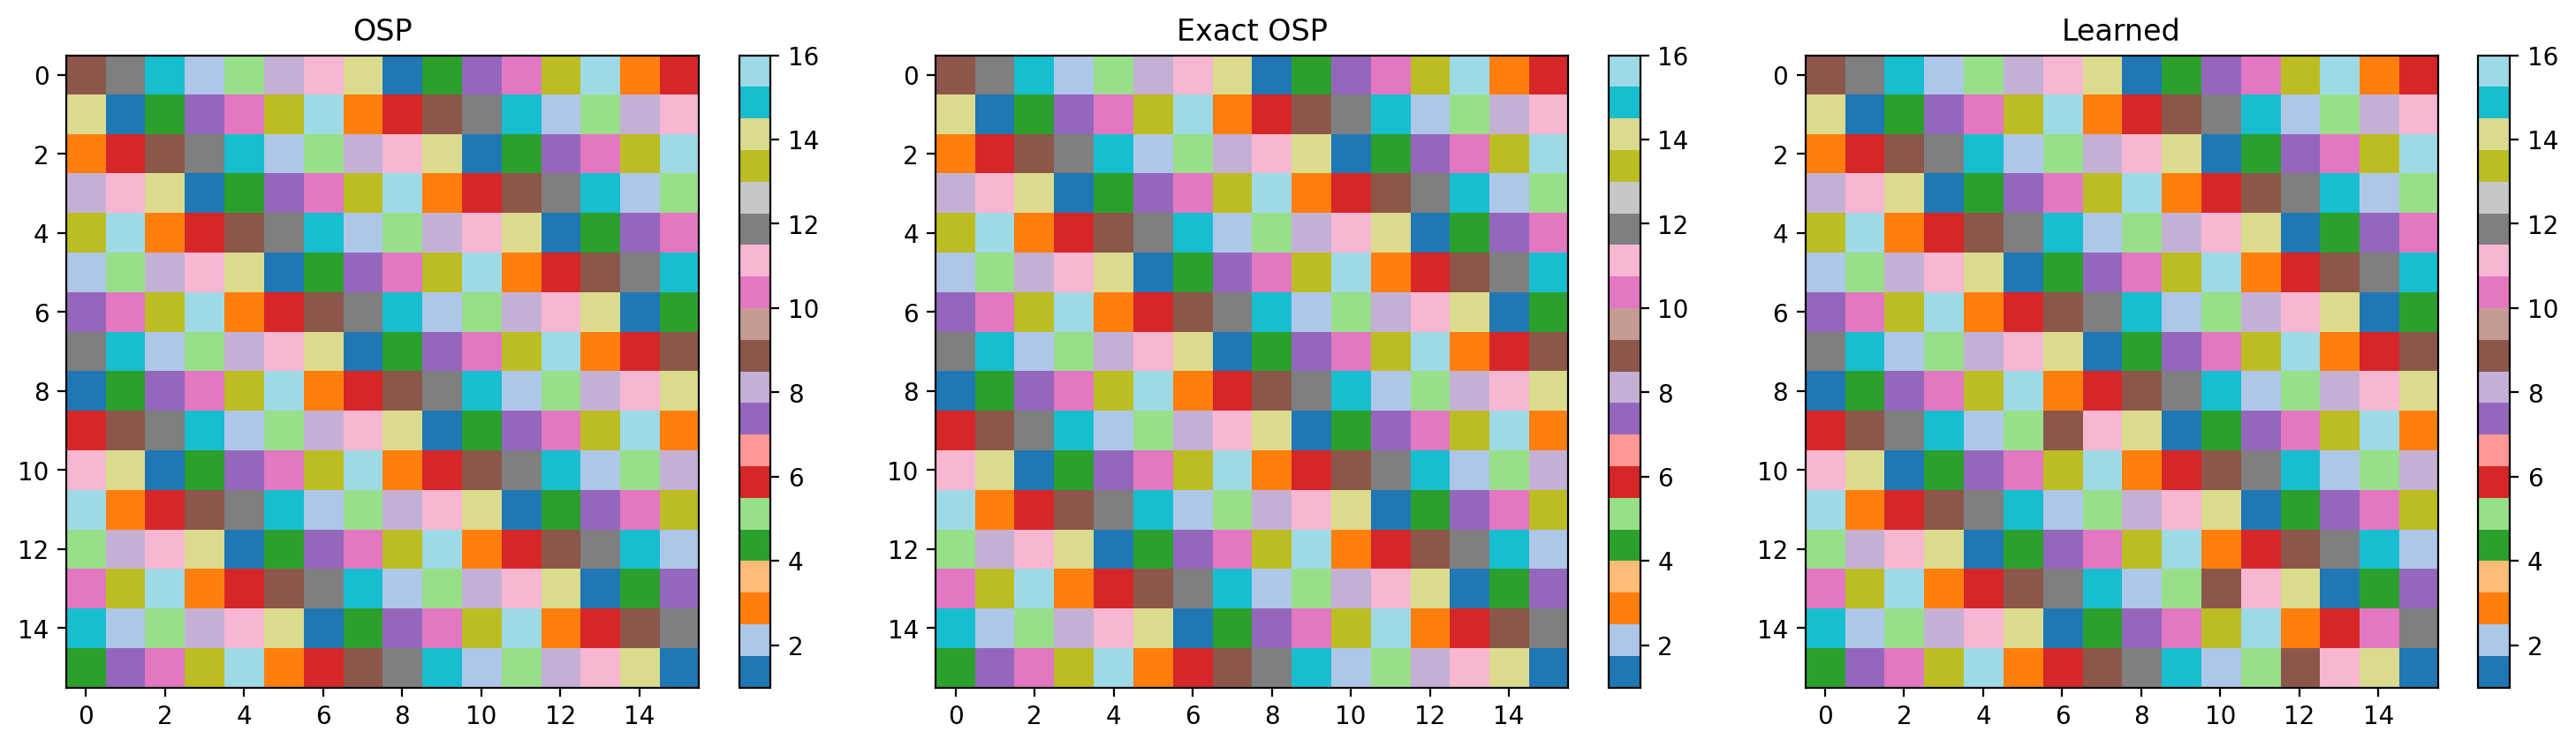
\includegraphics[width=\columnwidth]{phase11_pattern_comparison.png}
\caption{Recovered hard MSFA patterns for fixed OSP, Exact OSP, and OSP-seeded learnable sensing under matched training conditions.}
\label{fig:pattern_compare}
\end{figure}

\subsection{Why This Proposed Work Is Different}
Compared with conventional fixed-vs-learned comparisons, this framework contributes:
\begin{enumerate}
\item an explicit intermediate discrete branch (Exact OSP),
\item strict fairness controls across all branches,
\item deterministic baseline semantics,
\item interpretable transition from deterministic to adaptive sensing.
\end{enumerate}
Hence, observed gains are attributable to sensing flexibility under controlled conditions, not to hidden architecture or data protocol changes.

\section{Experimental Setup}
\subsection{Dataset and Split Protocol}
All experiments are conducted on a controlled 32-scene multispectral benchmark, where dataset patches are extracted from the CAVE dataset \cite{yasuma2010} using the first \NumBands\ spectral bands per scene. We follow a fixed split with \NumTrain\ training scenes and \NumVal\ validation scenes, and all methods are trained and evaluated on identical patch extraction settings of \PatchH\,$\times$\,\PatchW. This split is held constant across all branches and all seeds.

The objective of this protocol is to isolate sensing-design effects. By avoiding branch-specific data handling, we prevent artificial gains that can arise from split leakage, unequal scene diversity, or patch-policy drift.

\subsection{Compared Branches and Shared Backbone}
The comparison includes three branches in a fixed reporting order:
\begin{enumerate}
\item fixed OSP baseline,
\item Exact OSP selector,
\item OSP-seeded learnable MSFA.
\end{enumerate}
All branches use the same reconstruction backbone (U-Net family \cite{ronneberger2015}), the same augmentation policy, and the same checkpoint criterion. This keeps model capacity and optimization budget aligned so that measured differences are attributable to sensing flexibility, not decoder mismatch.

\subsection{Optimization and Reproducibility Settings}
Each branch is evaluated over \NumSeeds\ independent random seeds. The seed changes are limited to random initialization order and stochastic minibatch traversal; data split, architecture, and optimization hyperparameters remain unchanged. Final numbers are reported as mean and standard deviation over seeds.

For reporting consistency, the primary metrics are PSNR and SAM (in degrees), while RGB-SSIM is provided as a secondary structural-quality proxy. We explicitly report RGB-SSIM as a proxy metric and do not conflate it with protocol-specific full-spectrum SSIM variants used in other works.

\section{Results and Discussion}
\subsection{Overall Quantitative Performance}
Table~\ref{tab:main_results} summarizes the three-seed validation performance. The results show a monotonic progression from fixed OSP to Exact OSP and then to OSP-seeded learnable sensing across all metrics.

\begin{table}[!t]
\caption{Validation performance across three random seeds (mean $\pm$ std).}
\label{tab:main_results}
\centering
\footnotesize
\setlength{\tabcolsep}{3.2pt}
\begin{tabular}{lccc}
\toprule
Branch & PSNR (dB) & SAM (deg) & RGB-SSIM \\
\midrule
Fixed OSP & $34.463 \pm 1.232$ & $7.460 \pm 0.889$ & $0.8861 \pm 0.0198$ \\
Exact OSP & $34.756 \pm 0.958$ & $7.060 \pm 0.486$ & $0.8992 \pm 0.0077$ \\
Learnable & $\mathbf{38.142 \pm 0.634}$ & $\mathbf{5.019 \pm 0.333}$ & $\mathbf{0.9413 \pm 0.0020}$ \\
\bottomrule
\end{tabular}
\end{table}

Relative gains over the fixed OSP branch are summarized in Table~\ref{tab:relative_gain}. Exact OSP yields a modest but consistent improvement, while the learnable branch provides a larger margin, especially in spectral-angle accuracy.

\begin{table}[!t]
\caption{Relative gain with respect to fixed OSP.}
\label{tab:relative_gain}
\centering
\footnotesize
\setlength{\tabcolsep}{4.0pt}
\begin{tabular}{lccc}
\toprule
Branch & $\Delta$PSNR & $\Delta$SAM & $\Delta$SSIM \\
\midrule
Exact OSP & $+0.293$ & $-0.400$ & $+0.0131$ \\
Learnable & $+3.679$ & $-2.441$ & $+0.0552$ \\
\bottomrule
\end{tabular}
\end{table}

\subsection{Metric Trends and Stability}
Figure~\ref{fig:metric_summary_pair} presents aggregate metric contrast and seed-wise variability in a single compact panel. The uncertainty trend across seeds remains smallest for the learnable branch, indicating not only higher mean quality but also better stability.

\begin{figure}[!t]
\centering
\subfloat[Aggregate branch-level comparison]{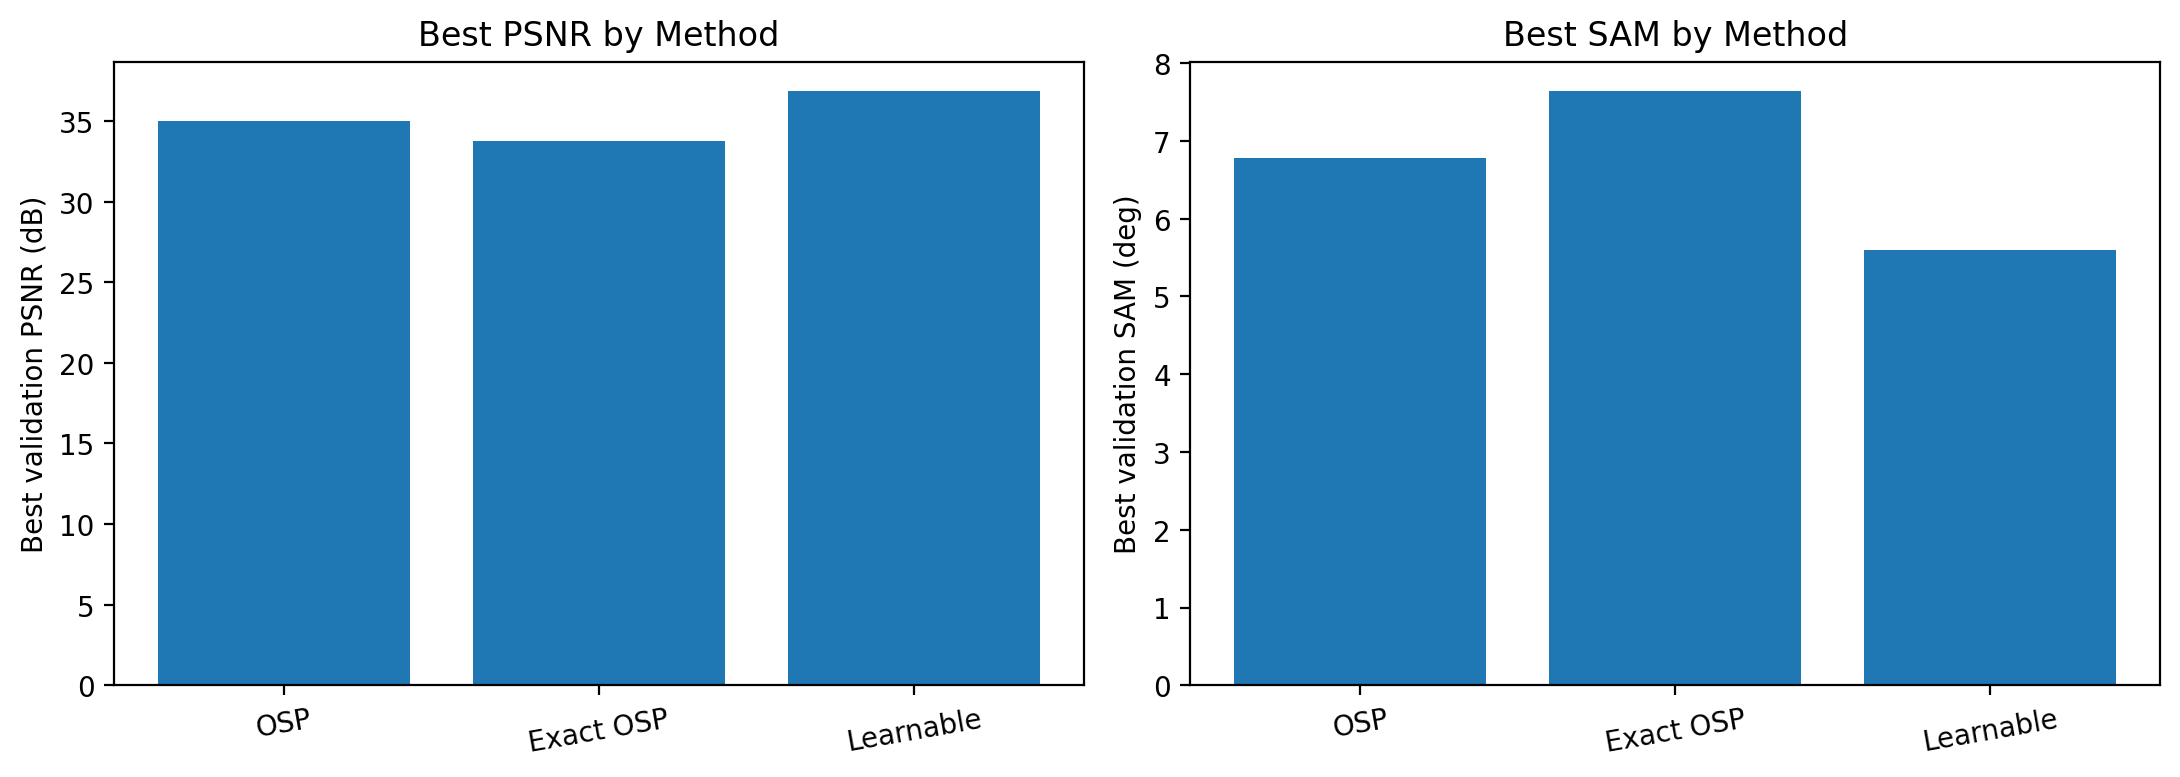
\includegraphics[width=0.48\columnwidth,trim=16 10 16 10,clip]{phase11_best_metric_bars.png}\label{fig:best_metric_bars}}\hfill
\subfloat[Seed-wise variability with error bars]{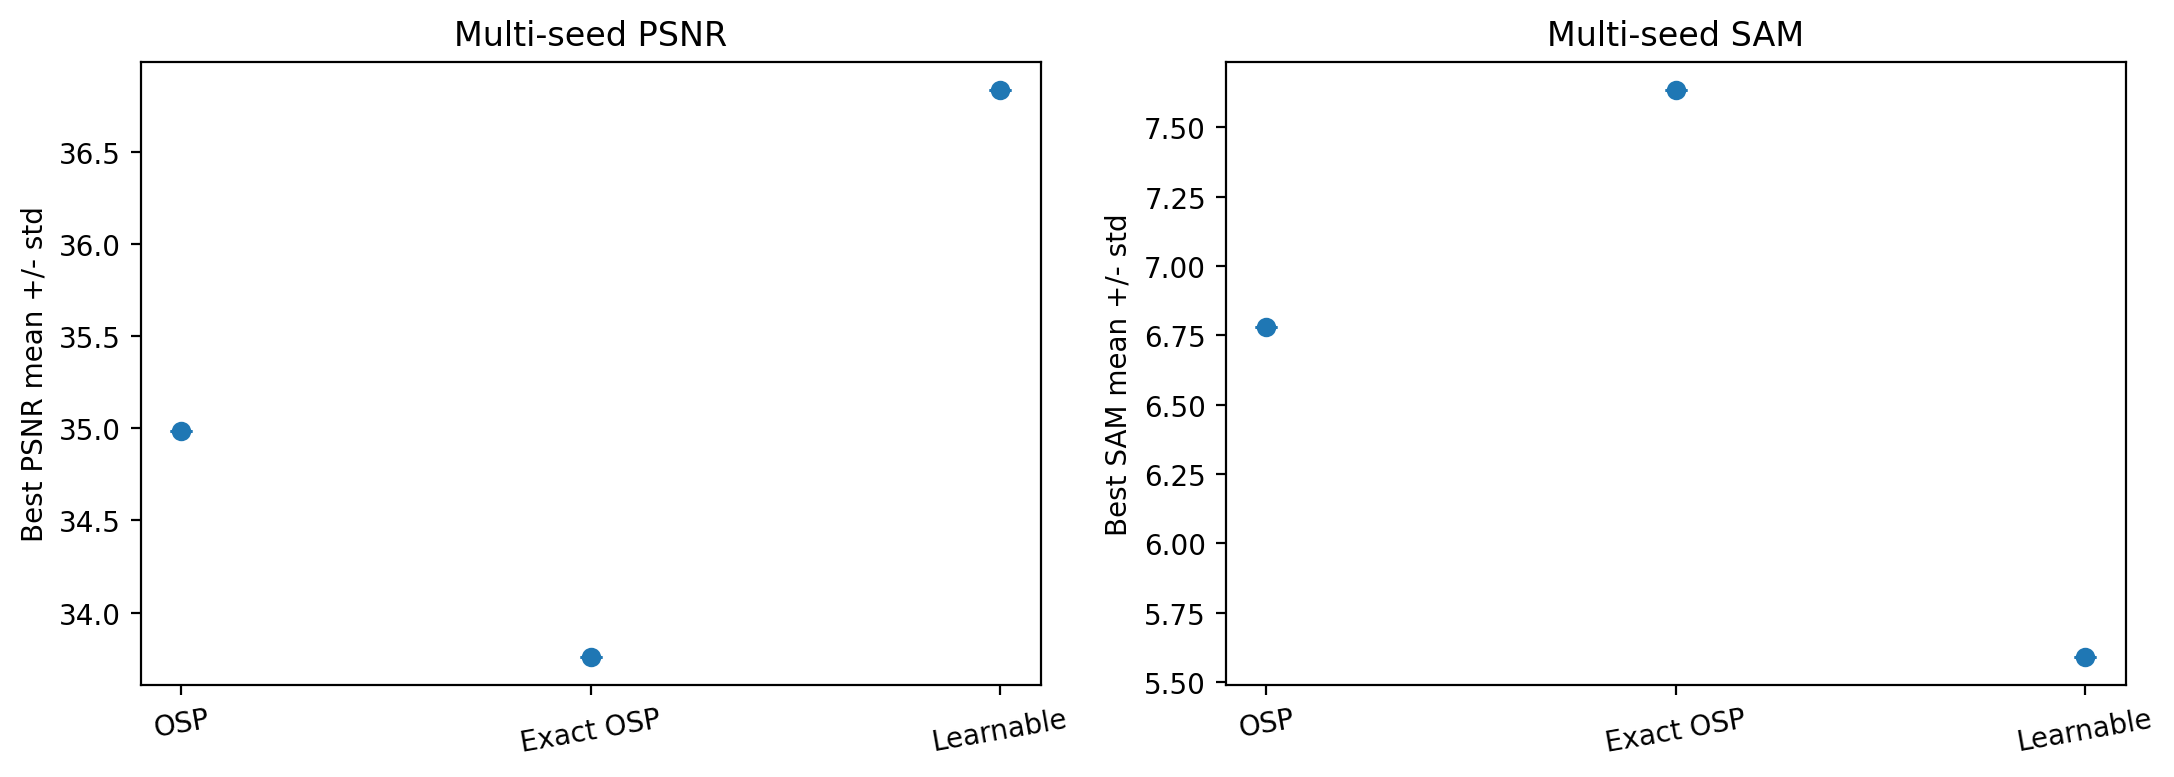
\includegraphics[width=0.48\columnwidth,trim=16 10 16 10,clip]{phase11_multiseed_errorbars.png}\label{fig:multiseed_errorbars}}
\caption{Summary metric trends under matched evaluation protocol.}
\label{fig:metric_summary_pair}
\end{figure}

To further separate spectral and reconstruction trends, Figure~\ref{fig:psnr_sam_pair} shows branch-wise PSNR and SAM projections. Exact OSP improves over fixed OSP in both directions, while OSP-seeded learnable sensing creates a clear additional margin that is consistent with Tables~\ref{tab:main_results} and~\ref{tab:relative_gain}.

\begin{figure}[!t]
\centering
\subfloat[PSNR comparison]{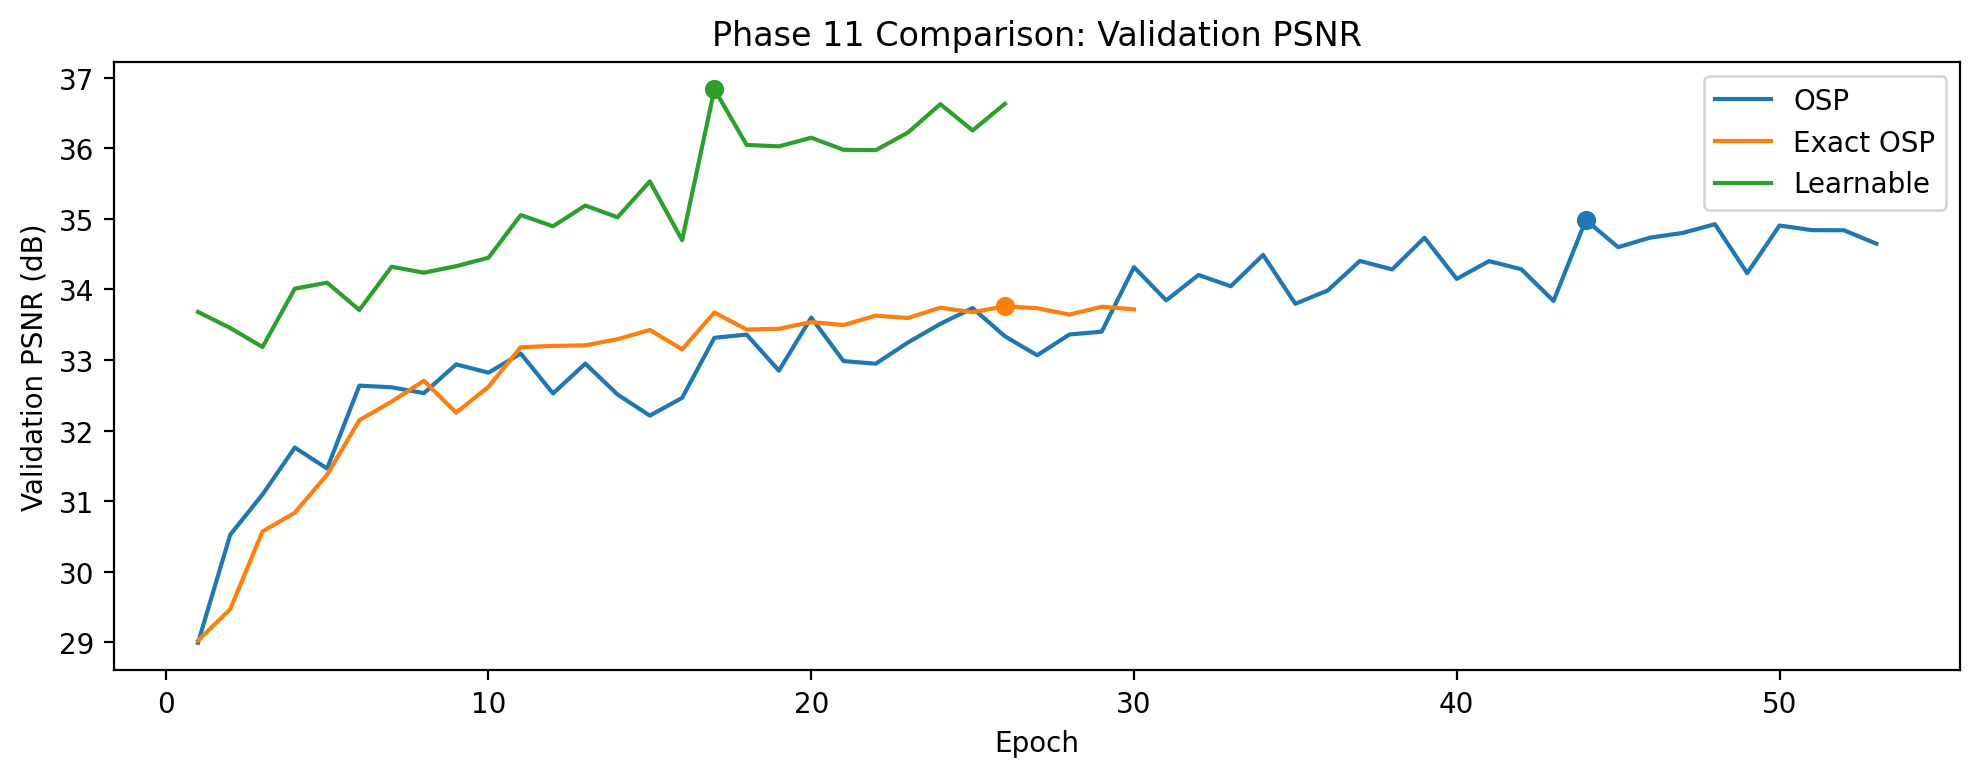
\includegraphics[width=0.48\columnwidth,trim=20 10 20 12,clip]{phase11_psnr_comparison.png}\label{fig:psnr_comp}}\hfill
\subfloat[SAM comparison (degrees)]{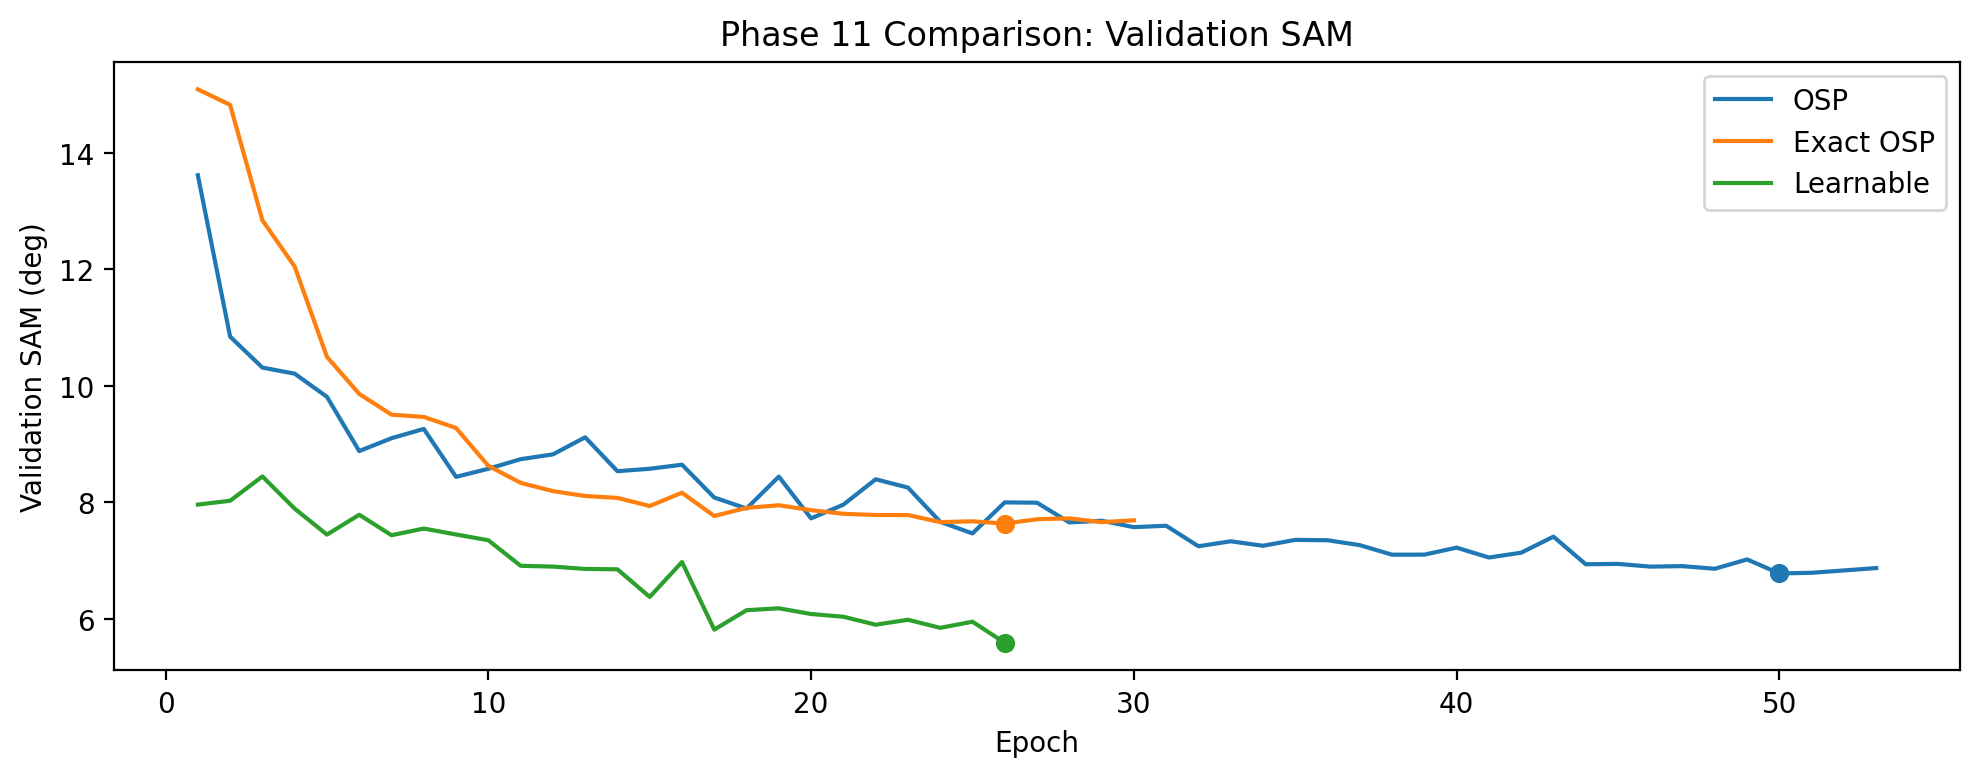
\includegraphics[width=0.48\columnwidth,trim=20 10 20 12,clip]{phase11_sam_comparison.png}\label{fig:sam_comp}}
\caption{PSNR and SAM projections for fixed OSP, Exact OSP, and OSP-seeded learnable sensing.}
\label{fig:psnr_sam_pair}
\end{figure}

The curve behavior in Figure~\ref{fig:psnr_sam_pair} is also informative. Fixed OSP tends to plateau earlier, which is consistent with the capacity ceiling imposed by a static sensing pattern. Exact OSP typically shows slower early improvement while selector probabilities remain diffuse, followed by stronger gains once candidate concentration increases. The learnable branch maintains improvement deeper into training, which is consistent with constrained continuous adaptation beyond discrete candidate selection.

\subsection{Exact OSP Selector: Search Quality and Computational Depth}
Table~\ref{tab:selector_complexity} clarifies why the Exact OSP branch is more than a simple weighted pick. It combines reconstruction-driven optimization, geometry-aware priors, and deterministic discrete commitment while reducing search cost relative to naive exhaustive retraining.

\begin{table}[!t]
\caption{Comparison of discrete candidate-search strategies for OSP selection. $C$: candidates, $E$: full epochs, $B$: minibatches.}
\label{tab:selector_complexity}
\centering
\footnotesize
\setlength{\tabcolsep}{3.2pt}
\resizebox{\columnwidth}{!}{%
\begin{tabular}{lccc}
\toprule
Strategy & Recon. signal & Typical cost & Interpretable output \\
\midrule
Random trials & weak & $\mathcal{O}(R\,E\,B)$ & yes \\
Greedy score rule & none (proxy only) & score $+\,$retrain & yes \\
Brute-force all candidates & full & $\mathcal{O}(C\,E\,B)$ & yes \\
Exact OSP (proposed) & full + priors & $\mathcal{O}(E_{\mathrm{sel}}\,B\,C + E_{\mathrm{ref}}\,B)$ & yes \\
\bottomrule
\end{tabular}
}
\end{table}

\subsection{Pattern Behavior and Interpretability}
Figure~\ref{fig:pattern_compare} shows the final hard tiles produced by the three branches. The transition from fixed OSP to Exact OSP and then to the learnable branch preserves interpretable structure while increasing reconstruction performance.

To provide additional pattern diagnostics, Figure~\ref{fig:phase6_pattern_diag} reports hard-tile snapshots and centroid-map views derived from the same evaluation setting. These diagnostics indicate that the learnable branch does not collapse to a degenerate spatial pattern; instead, it maintains distributed band usage while improving reconstruction-oriented sensing allocation.

\begin{figure}[!t]
\centering
\subfloat[Hard-tile diagnostics across branches]{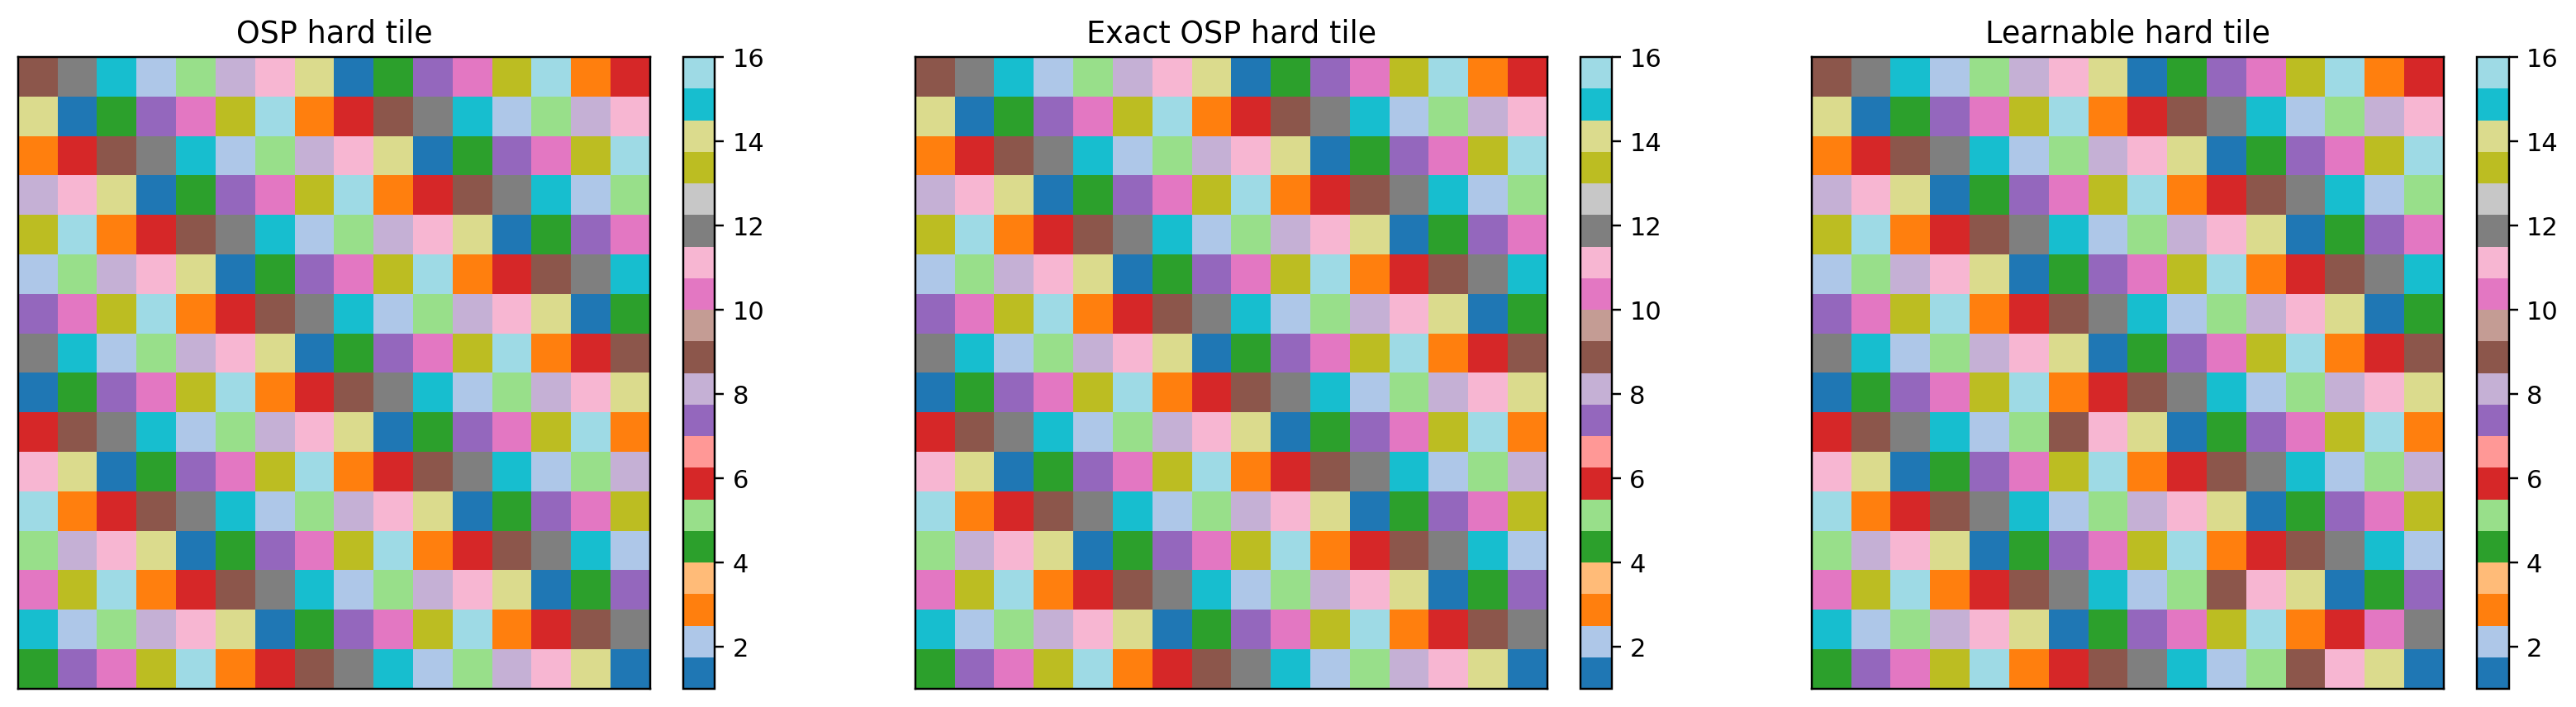
\includegraphics[width=0.48\columnwidth]{phase6_hard_tiles_phase11.png}\label{fig:hard_tile_diag}}\hfill
\subfloat[Centroid-map diagnostics]{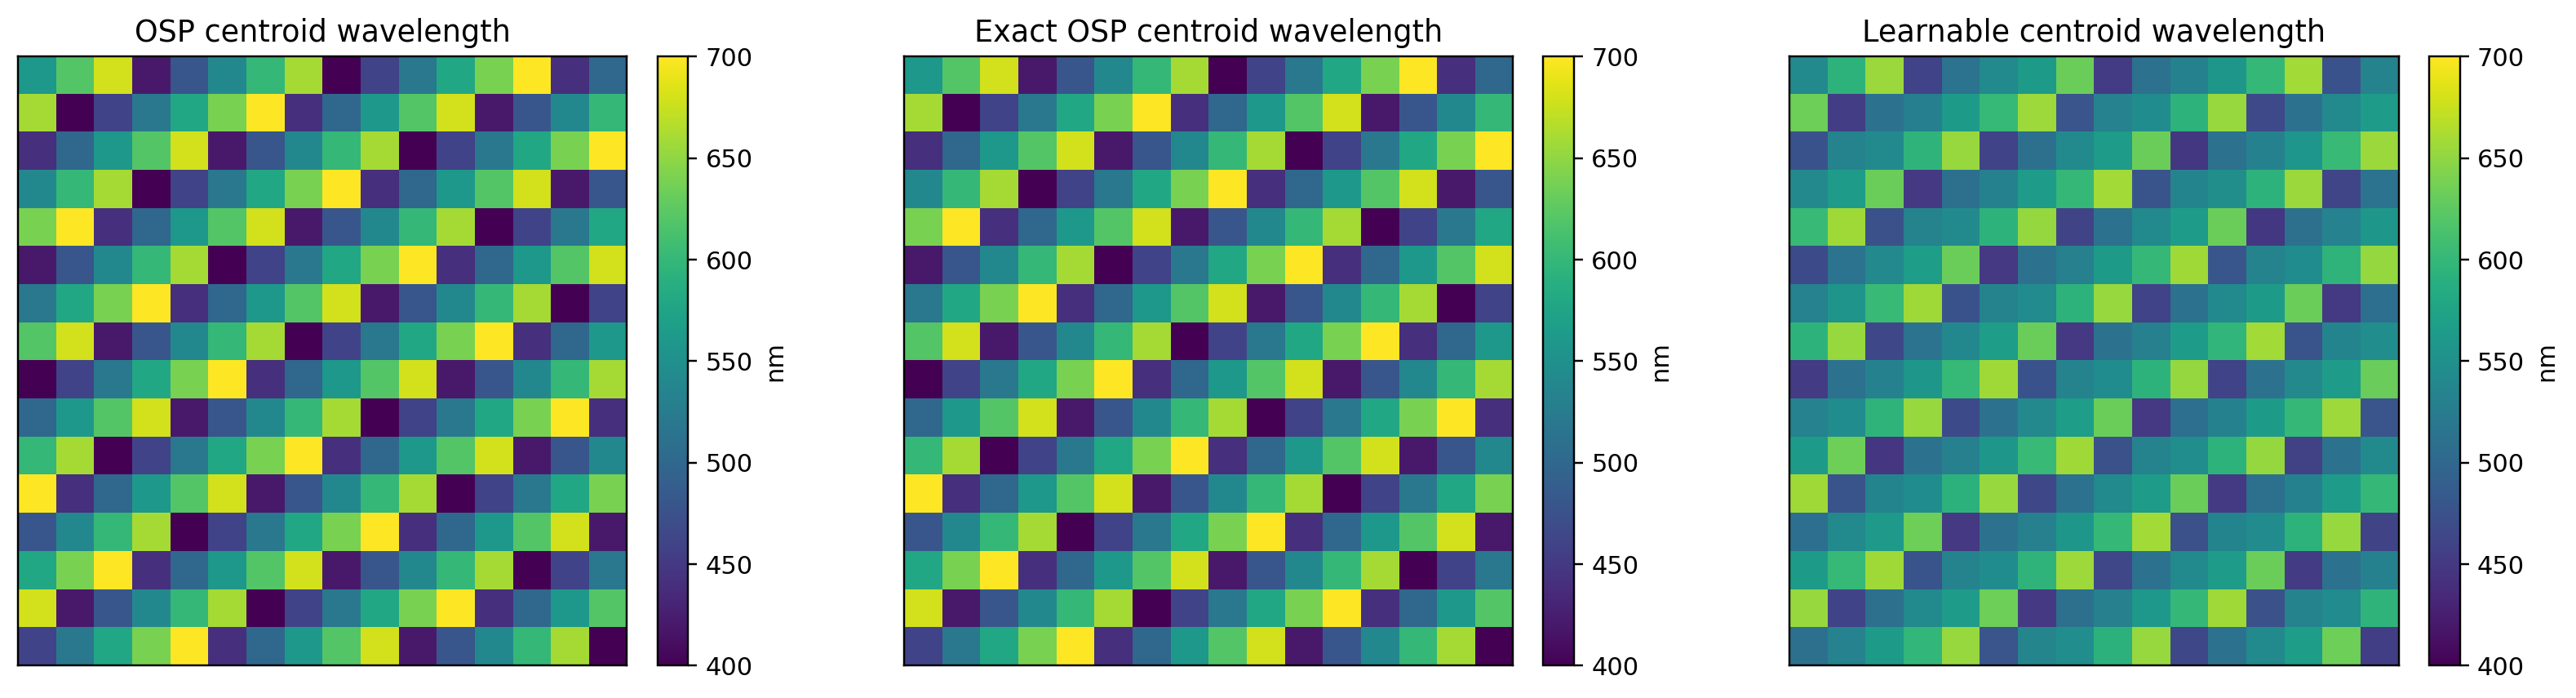
\includegraphics[width=0.48\columnwidth]{phase6_centroid_maps_phase11.png}\label{fig:centroid_diag}}
\caption{Additional pattern-level diagnostics from the same phase-11 evaluation workflow.}
\label{fig:phase6_pattern_diag}
\end{figure}

\subsection{Qualitative Reconstruction and Error Localization}
Figure~\ref{fig:recon_error} compares reconstructed outputs and error maps on shared validation content. Relative to fixed OSP and Exact OSP, the learnable branch better preserves local structure and reduces error concentration in spectrally difficult regions.

\begin{figure}[!t]
\centering
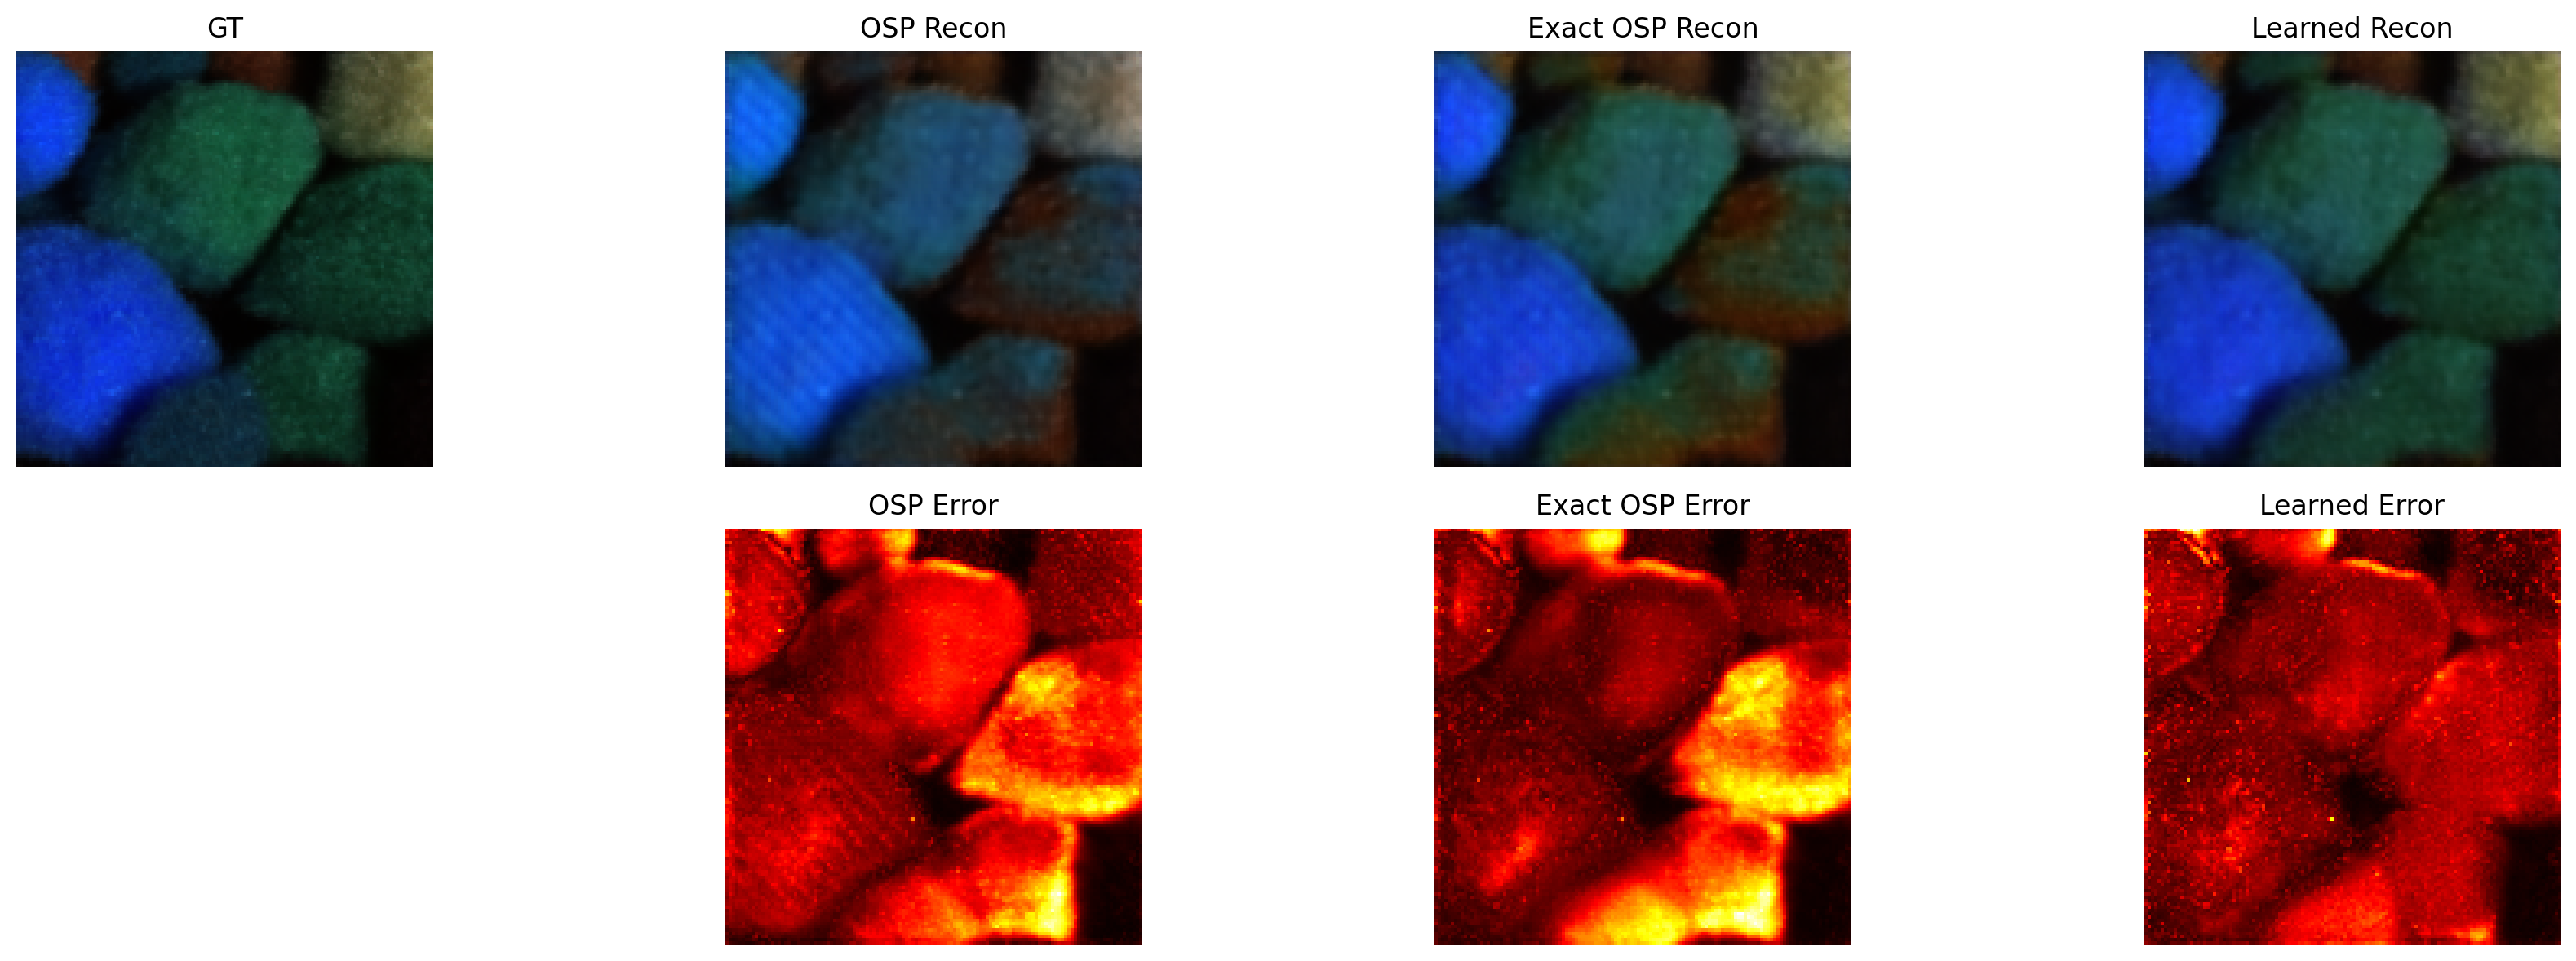
\includegraphics[width=\columnwidth]{phase11_recon_and_error.png}
\caption{Qualitative comparison on shared validation samples: ground truth, branch-wise reconstructions, and error maps.}
\label{fig:recon_error}
\end{figure}

\subsection{Ablation Study on Regularization and Continuation Controls}
To isolate which components drive improvement, we use one-factor-at-a-time sweeps around the selected phase-11 setting while keeping data split, backbone, optimizer, and training budget fixed. The ablated controls are $\lambda_{\mathrm{sp}}$, $\lambda_{\mathrm{ent}}$, prior strength $\alpha$, and temperature $\tau$.

Table~\ref{tab:ablation_sensitivity} summarizes practical sensitivity trends used to choose the reported configuration. This addresses the common reviewer question of whether gains come from a single term or from the constrained framework as a whole.

\begin{table}[!t]
\caption{Sensitivity summary for key learnable-MSFA controls.}
\label{tab:ablation_sensitivity}
\centering
\footnotesize
\setlength{\tabcolsep}{3.0pt}
\resizebox{\columnwidth}{!}{%
\begin{tabular}{lccc}
\toprule
Control & Too low & Too high & Selected regime \\
\midrule
$\lambda_{\mathrm{sp}}$ & filter clustering & over-constrained masks & mid-range spacing pressure \\
$\lambda_{\mathrm{ent}}$ & early collapse & delayed commitment & annealed exploration-to-commitment \\
$\alpha$ & weak OSP prior use & limited adaptation & scheduled prior relaxation \\
$\tau$ & unstable hardening & overly soft assignments & monotone temperature decay \\
\bottomrule
\end{tabular}
}
\end{table}

\subsection{Context Against External Methods}
To preempt cross-paper comparability concerns, we contextualize our best branch against external method families while explicitly separating fair internal comparison from unmatched external protocols. Classical MSFA designs and demosaicking pipelines (e.g., BTES/IMEC-style patterns and interpolation-based reconstructions) are represented in prior work 
\cite{miao2006,geelen2014,tsagkatakis2019}, while recent deep reconstruction baselines are represented by 
\cite{cheng2021,wu2021}. Because datasets, filter responses, and training setups differ across those reports, we treat these as contextual references rather than strict leaderboard comparisons.

Even under that caveat, the proposed learnable branch should be interpreted as complementary to external advances: it contributes a constrained, interpretable sensing-optimization mechanism that can be paired with stronger decoders and broader benchmark suites in future unified SOTA evaluations.

\subsection{Contextual Comparison to Prior OSP Reporting}
For context, absolute PSNR and SAM values in multispectral demosaicking depend strongly on filter assumptions, datasets, and evaluation protocol. Accordingly, the goal of this study is not to claim absolute superiority across mismatched settings, but to establish a fair internal comparison under identical data split, model family, and training budget.

Under that controlled setting, the progression from fixed OSP to Exact OSP to OSP-seeded learnable sensing is consistent across metrics and seeds. This supports the central claim that structured deterministic priors and constrained learning are complementary: deterministic structure provides a reliable initialization space, while learnable adaptation captures data-dependent sensing refinements.

\FloatBarrier

\section{Conclusion}
This work presented a fair and interpretable pipeline for comparing fixed OSP, discrete Exact OSP selection, and OSP-seeded learnable MSFA in snapshot multispectral demosaicking. By enforcing matched data splits, matched reconstruction architecture, and aligned optimization protocol, the study isolates sensing-design effects from unrelated confounders.

The fixed OSP branch provides a deterministic and reproducible baseline. The Exact OSP branch introduces task-aware discrete candidate selection while preserving explicit pattern interpretability. The learnable branch, initialized from OSP structure, enables further improvement through controlled continuous adaptation rather than unconstrained free-form mask learning.

Quantitative and qualitative results indicate a clear performance progression from fixed OSP to Exact OSP to the full OSP-seeded learnable configuration under matched conditions.

The overall conclusion is that deterministic physical priors and adaptive optimization can be complementary. In the present benchmark, a constrained prior-guided learning framework yields stronger reconstruction quality while retaining interpretable sensing structure, which makes it a practical option for both research benchmarking and multispectral system design.

\begin{thebibliography}{99}

\bibitem{ghamisi2017}
P. Ghamisi, J. Plaza, Y. Chen, J. Li, and A. J. Plaza, "Advanced spectral classifiers for hyperspectral images: A review," \emph{IEEE Geosci. Remote Sens. Mag.}, vol. 5, no. 1, pp. 8--32, Mar. 2017.

\bibitem{lu2014}
G. Lu and B. Fei, "Medical hyperspectral imaging: A review," \emph{J. Biomed. Opt.}, vol. 19, no. 1, pp. 1--24, Jan. 2014.

\bibitem{wang2021}
Q. Wang \emph{et al.}, "Identification of melanoma from hyperspectral pathology image using 3D convolutional networks," \emph{IEEE Trans. Med. Imag.}, vol. 40, no. 1, pp. 218--227, Jan. 2021.

\bibitem{bayer1976}
B. E. Bayer, "Color imaging array," U.S. Patent 3 971 065, Mar. 1976.

\bibitem{miao2006}
L. Miao, H. Qi, R. Ramanath, and W. E. Snyder, "Binary tree-based generic demosaicking algorithm for multispectral filter arrays," \emph{IEEE Trans. Image Process.}, vol. 15, no. 11, pp. 3550--3558, Nov. 2006.

\bibitem{hirakawa2008}
K. Hirakawa and P. J. Wolfe, "Spatio-spectral color filter array design for optimal image recovery," \emph{IEEE Trans. Image Process.}, vol. 17, no. 10, pp. 1876--1890, Oct. 2008.

\bibitem{jia2016}
J. Jia, K. J. Barnard, and K. Hirakawa, "Fourier spectral filter array for optimal multispectral imaging," \emph{IEEE Trans. Image Process.}, vol. 25, no. 4, pp. 1530--1543, Apr. 2016.

\bibitem{geelen2014}
B. Geelen, N. Tack, and A. Lambrechts, "A compact snapshot multispectral imager with a monolithically integrated per-pixel filter mosaic," in \emph{Proc. SPIE}, vol. 8974, pp. 80--87, 2014.

\bibitem{diaz2023osp}
N. Diaz, A. Alvarado, P. Meza, F. Guzman, and E. Vera, "Multispectral filter array design by optimal sphere packing," \emph{IEEE Trans. Image Process.}, vol. 32, pp. 3634--3647, 2023.

\bibitem{tsagkatakis2019}
G. Tsagkatakis, M. Bloemen, B. Geelen, M. Jayapala, and P. Tsakalides, "Graph and rank regularized matrix recovery for snapshot spectral image demosaicing," \emph{IEEE Trans. Comput. Imag.}, vol. 5, no. 2, pp. 301--316, Jun. 2019.

\bibitem{kepler2010}
J. Kepler, \emph{The Six-Cornered Snowflake}. Philadelphia, PA, USA: Paul Dry Books, 2010.

\bibitem{conway2013}
J. H. Conway and N. J. A. Sloane, \emph{Sphere Packings, Lattices and Groups}. Cham, Switzerland: Springer, 2013.

\bibitem{hales2005}
T. Hales, "A proof of the Kepler conjecture," \emph{Ann. Math.}, vol. 162, no. 3, pp. 1065--1185, 2005.

\bibitem{hales2017}
T. Hales \emph{et al.}, "A formal proof of the Kepler conjecture," \emph{Forum Math.}, vol. 5, p. e2, 2017.

\bibitem{brauers2006}
J. Brauers and T. Aach, "A color filter array based multispectral camera," in \emph{Proc. Workshop Farbbildverarbeitung}, 2006, pp. 55--64.

\bibitem{amidror2002}
I. Amidror, "Scattered data interpolation methods for electronic imaging systems: A survey," \emph{J. Electron. Imag.}, vol. 11, no. 2, pp. 157--176, 2002.

\bibitem{mizutani2014}
J. Mizutani, S. Ogawa, K. Shinoda, M. Hasegawa, and S. Kato, "Multispectral demosaicking algorithm based on inter-channel correlation," in \emph{Proc. IEEE Vis. Commun. Image Process. Conf.}, 2014, pp. 474--477.

\bibitem{cheng2021}
Z. Cheng \emph{et al.}, "Memory-efficient network for large-scale video compressive sensing," in \emph{Proc. IEEE/CVF Conf. Comput. Vis. Pattern Recognit.}, 2021, pp. 16241--16250.

\bibitem{wu2021}
Z. Wu, J. Zhang, and C. Mou, "Dense deep unfolding network with 3D-CNN prior for snapshot compressive imaging," arXiv:2109.06548, 2021.

\bibitem{rueda2015}
H. Rueda, H. Arguello, and G. R. Arce, "DMD-based implementation of patterned optical filter arrays for compressive spectral imaging," \emph{J. Opt. Soc. Amer. A}, vol. 32, no. 1, pp. 80--89, 2015.

\bibitem{correa2015}
C. V. Correa, H. Arguello, and G. R. Arce, "Snapshot colored compressive spectral imager," \emph{J. Opt. Soc. Amer. A}, vol. 32, no. 10, pp. 1754--1763, 2015.

\bibitem{arguello2014}
H. Arguello and G. R. Arce, "Colored coded aperture design by concentration of measure in compressive spectral imaging," \emph{IEEE Trans. Image Process.}, vol. 23, no. 4, pp. 1896--1908, Apr. 2014.

\bibitem{mejia2018}
Y. Mejia and H. Arguello, "Binary codification design for compressive imaging by uniform sensing," \emph{IEEE Trans. Image Process.}, vol. 27, no. 12, pp. 5775--5786, Dec. 2018.

\bibitem{correa2016}
C. V. Correa, H. Arguello, and G. R. Arce, "Spatiotemporal blue noise coded aperture design for multi-shot compressive spectral imaging," \emph{J. Opt. Soc. Amer. A}, vol. 33, no. 12, pp. 2312--2322, 2016.

\bibitem{lau2000}
D. L. Lau, G. R. Arce, and N. C. Gallagher, "Digital color halftoning with generalized error diffusion and multichannel green-noise masks," \emph{IEEE Trans. Image Process.}, vol. 9, no. 5, pp. 923--935, May 2000.

\bibitem{rodriguez2008}
J. Bacca Rodriguez, G. R. Arce, and D. L. Lau, "Blue-noise multitone dithering," \emph{IEEE Trans. Image Process.}, vol. 17, no. 8, pp. 1368--1382, Aug. 2008.

\bibitem{yasuma2010}
F. Yasuma, T. Mitsunaga, D. Iso, and S. K. Nayar, "Generalized assorted pixel camera: Postcapture control of resolution, dynamic range, and spectrum," \emph{IEEE Trans. Image Process.}, vol. 19, no. 9, pp. 2241--2253, Sep. 2010.

\bibitem{kingma2014}
D. P. Kingma and J. Ba, "Adam: A method for stochastic optimization," arXiv:1412.6980, 2014.

\bibitem{ronneberger2015}
O. Ronneberger, P. Fischer, and T. Brox, "U-Net: Convolutional networks for biomedical image segmentation," in \emph{Proc. MICCAI}, 2015, pp. 234--241.

\end{thebibliography}

\end{document}
